\documentclass[14pt,a4paper]{extarticle}

\usepackage[utf8]{inputenc}
\usepackage[T2A]{fontenc}
\usepackage{amssymb,amsmath,mathrsfs,amsthm}
\usepackage[russian]{babel}
\usepackage{graphicx}
\usepackage[footnotesize]{caption2}
\usepackage{indentfirst}
\usepackage{multicol}
\usepackage{listings}
\usepackage{float}
\usepackage{url}

\usepackage{enumitem}

%\usepackage[ruled,section]{algorithm}
%\usepackage[noend]{algorithmic}
%\usepackage[all]{xy}
\usepackage{booktabs}
\usepackage{graphicx}
\usepackage[table,xcdraw]{xcolor}
\usepackage{tcolorbox}

%Библиотека для блок-схем
\usepackage{tikz}
\usetikzlibrary{shapes,arrows}

% Параметры страницы
\textheight=24cm
\textwidth=16cm
\oddsidemargin=5mm
\evensidemargin=-5mm
\marginparwidth=36pt
\topmargin=-1cm
\footnotesep=3ex
%\flushbottom
\raggedbottom
\tolerance 3000
% подавить эффект "висячих стpок"
\clubpenalty=10000
\widowpenalty=10000
%\renewcommand{\baselinestretch}{1.1}
\renewcommand{\baselinestretch}{1.5} %для печати с большим интервалом

\newcommand{\angstrom}{\mbox{\normalfont\AA}}

\newtheorem{definition}{Определение} % задаём выводимое слово (для определений)
\newtheorem{example}{Замечание} % задаём выводимое слово (для определений)
\newtheorem{theorem}{Теорема} % задаём выводимое слово (для определений)
\newtheorem{proposition}{Утверждение} % задаём выводимое слово (для определений)
\newtheorem{construction}{Конструкция} % задаём выводимое слово (для определений)

\DeclareMathOperator*{\sgn}{sgn}
\DeclareMathOperator*{\var}{var}
\DeclareMathOperator*{\cov}{cov}
\DeclareMathOperator*{\law}{Law}

\newcommand{\1}{\mathbbm{1}}
\newcommand{\R}{\mathbb{R}}
\newcommand{\N}{\mathbb{N}}
\newcommand{\Z}{\mathbb{Z}}
\renewcommand{\P}{\mathbb{P}}
\newcommand{\E}{\mathbb{E}}

\newcommand{\independent}{\perp\!\!\!\!\perp}

\newcommand\cA{{\cal A}}
\newcommand\cE{{\cal E}}
\newcommand\cC{{\cal C}}
\newcommand\cF{{\cal F}}
\newcommand\cG{{\cal G}}
\newcommand\cK{{\cal K}}
\newcommand\cL{{\cal L}}
\newcommand\cB{{\cal B}}
\newcommand\cN{{\cal N}}
\newcommand\cM{{\cal M}}
\newcommand\cX{{\cal X}}
\newcommand\cD{{\cal D}}
\newcommand\cR{{\cal R}}
\newcommand\cP{{\cal P}}
\newcommand\cQ{{\cal Q}}
\newcommand\cS{{\cal S}}
\newcommand\cT{{\cal T}}
\newcommand\cV{{\cal V}}
\newcommand\cZ{{\cal Z}}

\newcommand{\textProposition}    {Предложение}
\newcommand{\textTask}    {Задача}

\begin{document}

\begin{center}

    {Всеволод Заостровский, 409 группа}\\
    {\bfseries Отчёт по задаче ''Численное решение дифференциальных уравнений второго порядка методами Фурье и прогонки''.\\}
    \vspace{1cm}

\end{center}

\section{Постановка задачи.} Необходимо решить уравнение:
\begin{equation} \label{diffeq1}
    -y'' + p(x) y(x) = f(x).
\end{equation}
В моём варианте, краевые условия:
\begin{align} \label{diffeqedge}
    & y_0 = 0, \quad y_N = 0, \quad h = \frac{1}{N}. \\
\end{align}

\section{Численная схема и её сходимость.}

Будем аппроксимировать дифференциальное уравнение схемой:
\begin{equation} \label{scheme1}
    -\frac{y_{k+1} - 2 y_k + y_{k-1}}{h^2} + p y_k = f_k, \quad k = 1, \ldots, N - 1;
\end{equation}
с краевыми условиями:
\begin{equation} \label{schemeedge}
    y_0 = y_N = 0,
    \quad h = \frac{1}{N}, 
    \quad p \geq 0.
\end{equation}
Исследуем сходимость схемы с помощью теоремы Филлипова.
\begin{theorem}
    \begin{enumerate}
        \item \eqref{diffeq1} и \eqref{scheme1} --- линейны.
        \item Существует единственное решение задачи \eqref{diffeq1} с краевыми условиями \eqref{diffeqedge}.
        \item Разностная схема \eqref{scheme1} аппроксимирует задачу на решении с порядком 2:
            \begin{equation*}
                || L_h [y]_h - f_h || _{2, h} \leq C h^2.           
            \end{equation*}
        \item Разностная схема устойчива в норме $||\cdot||_{2,h}$:
        \begin{equation*}
            || A^{-1} ||_{2,h} \leq \text{const}.
        \end{equation*}
    \end{enumerate}
\end{theorem}

\begin{proposition}
    Теорема Филлипова выполняется для задачи \eqref{diffeq1}--\eqref{diffeqedge} и схемы \eqref{scheme1}--\eqref{schemeedge}.
\end{proposition}
\begin{proof}
    \begin{enumerate}
        \item  \eqref{diffeq1} и \eqref{scheme1} --- линейны по определению.
        \item Из теории дифференциальных уравнений известно, что такой тип уравнений имеет единственное решение.
        \item По определению аппроксимации на решении,
        \begin{align*}
            & || L_h [y]_h - f_h || _{2, h} = || -\frac{y(x_{k+1}) - 2 y(x_k) + y(x_{k-1})}{h^2} + p y_k - f(x_k) || _{2, h} = \\ 
            & =|| -\frac{1}{h^2}\left(y(x_{k}) + h y'(x_{k}) + \frac{h^2}{2} y''(x_{k}) + \frac{h^3}{6} y'''(x_{k}) + O(h^4)\right)  \\
            & -\frac{1}{h^2}\left(y(x_{k}) - h y'(x_{k}) + \frac{h^2}{2} y''(x_{k}) - \frac{h^3}{6} y'''(x_{k}) + O(h^4)\right) \\ 
            & + p y_k + \frac{2}{h^2} y(x_k) - f(x_k) || _{2, h} = || O(h^2) + \underbrace{(- y''(x_{k}) + p y_k - f(x_k))}_{=0 \text{, поскольку $y$ --- решение}} ||_{2, h} \leq C h^2 \\ .           
        \end{align*}
        При этом краевые условия даны точно. Таким образом, имеем 2 порядок аппроксимации на решении.
        \item В отчёте к задаче по итерационным методам решения систем уравнений (см. каталог LinAlg) были найдены собственные значения 
        (и собственные векторы) задачи выше (при условии, что $p = \text{const}$): 
        \begin{equation*}
            \lambda_n = p - 2 N^2 (\cos(\frac{\pi n}{N}) - 1) = \frac{4}{h^2} \sin^2(\frac{\pi n h}{2}) + p.
        \end{equation*}
        Поскольку $sin x \geq \frac{2}{\pi} x $ при $x \leq \frac{\pi}{2}$, для собственных значений имеем оценку:
        \begin{equation*}
            \lambda_n = \frac{4}{h^2} \sin^2(\frac{\pi n h}{2}) + p \geq \frac{4}{h^2} \frac{4}{\pi ^2} \frac{\pi ^2 n^2 h^2}{4} + p > \text{const} > 0.
        \end{equation*}
        Тогда
        \begin{equation*}
            || A^{-1} ||_{2,h} = max \frac{1}{\lambda(A)} \leq \text{const}.
        \end{equation*}
    \end{enumerate}
    Таким образом, по теореме Филлипова, схема имеет порядок сходимости равный двум.
\end{proof}

\section{Програмная релизация решения дифференциального уравнения.}
Для численной реализации схемы фактически необходимо решить систему уравнений \eqref{scheme1}--\eqref{schemeedge}. 
В случае постоянного $p$ это можно сделать методом Фурье. В более общем случае --- методом прогонки. Были реализованы оба метода. См. папку /../Code/src .
\subsection{Порядок сходимости схемы.}
Поскольку схема имеет второй порядок сходимости, она должна быть точна на полиномах до 2 степени включительно. Рассмотрим задачу
\begin{equation*} \label{diffeq1}
    -y'' = 1,
\end{equation*}
с краевыми условиями:
\begin{align*} \label{diffeqedge}
    & y(0) = 0, \quad y(1) = 0. \\
\end{align*}
Её решение: $y = \frac{-x(x-1)}{2}$. Решим эту задачу численно на небольшом количестве точек. Как видно из рисунков, графики точно совпали 
(это проверено численно, точки совпадают с машинной точностью).
\begin{figure}
    \centering
    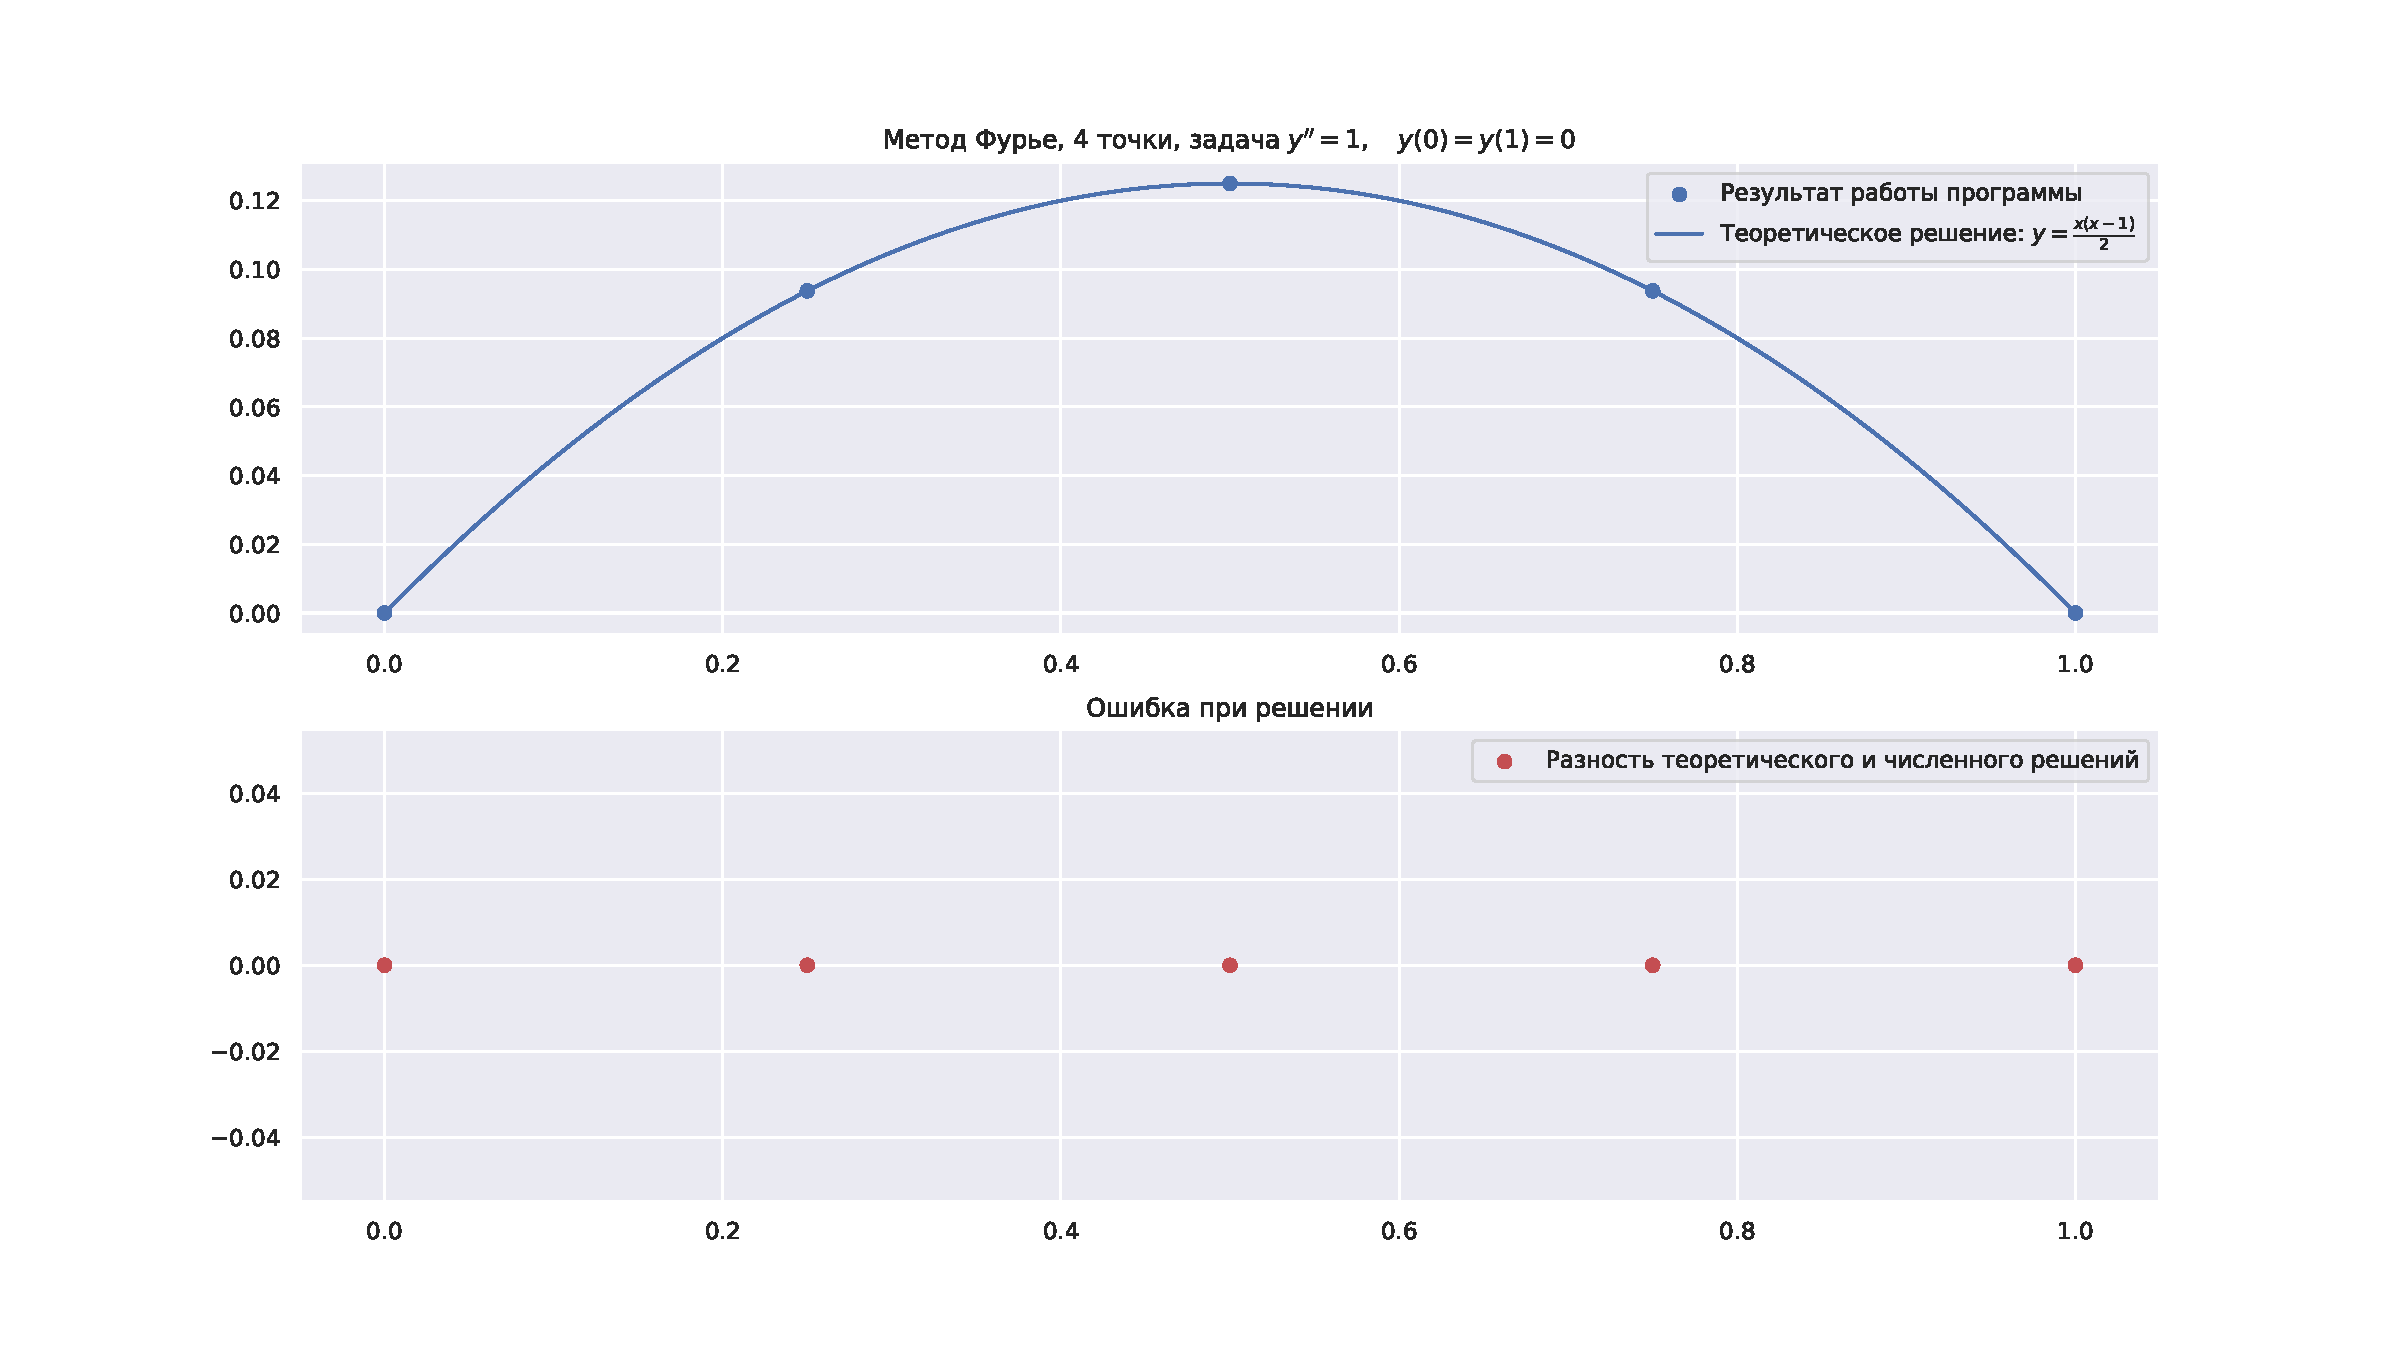
\includegraphics[scale=0.4]{figs/f4p0f1.pdf}
    \caption{Результаты теста на порядок сходимости для $p=0$, метод Фурье}
\end{figure}

\begin{figure}
    \centering
    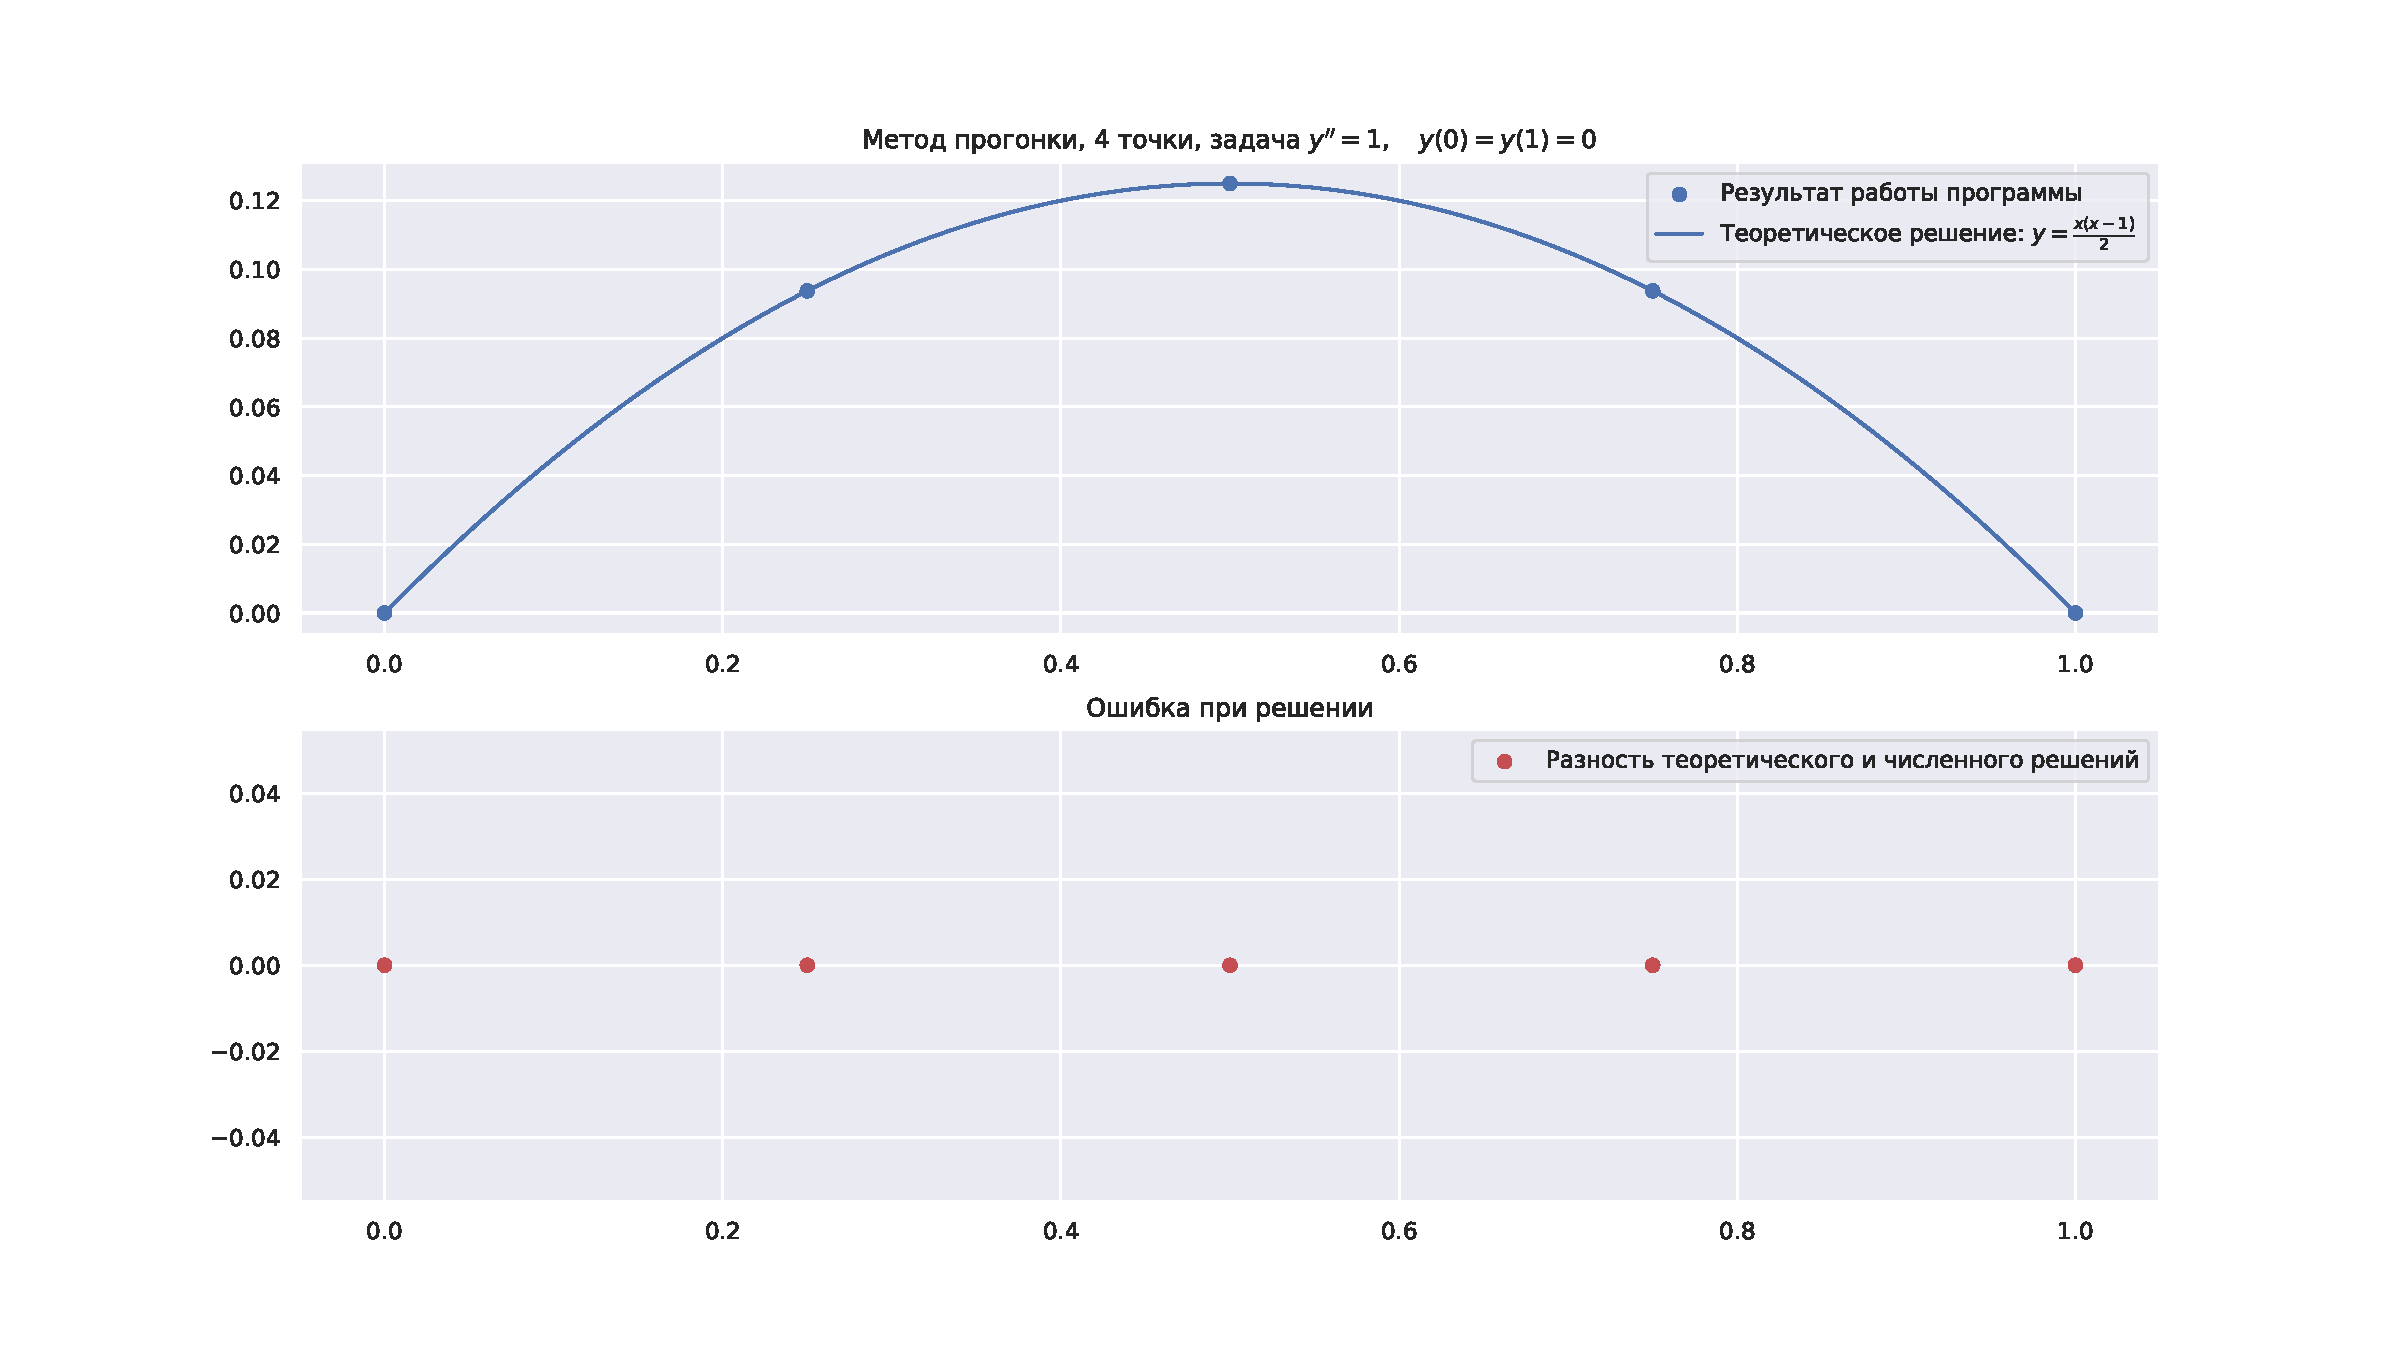
\includegraphics[scale=0.4]{figs/s4p0f1.pdf}
    \caption{Результаты теста на порядок сходимости для $p=0$, метод прогонки}
\end{figure}

\subsection{Корректность работы с $p\neq0$.}
Теперь рассмотрим задачу
\begin{equation*} \label{diffeq1}
    -y'' + y = 1,
\end{equation*}
с краевыми условиями:
\begin{align*} \label{diffeqedge}
    & y(0) = 0, \quad y(1) = 0. \\
\end{align*}
Её решение: $y = C e^x - (1 + C) e^{-t} + 1$, где $C = -\frac{1}{e + 1}$. Погрешность численного решения не видна на графике. Она составляет примерно $3e-6$.
\begin{figure}
    \centering
    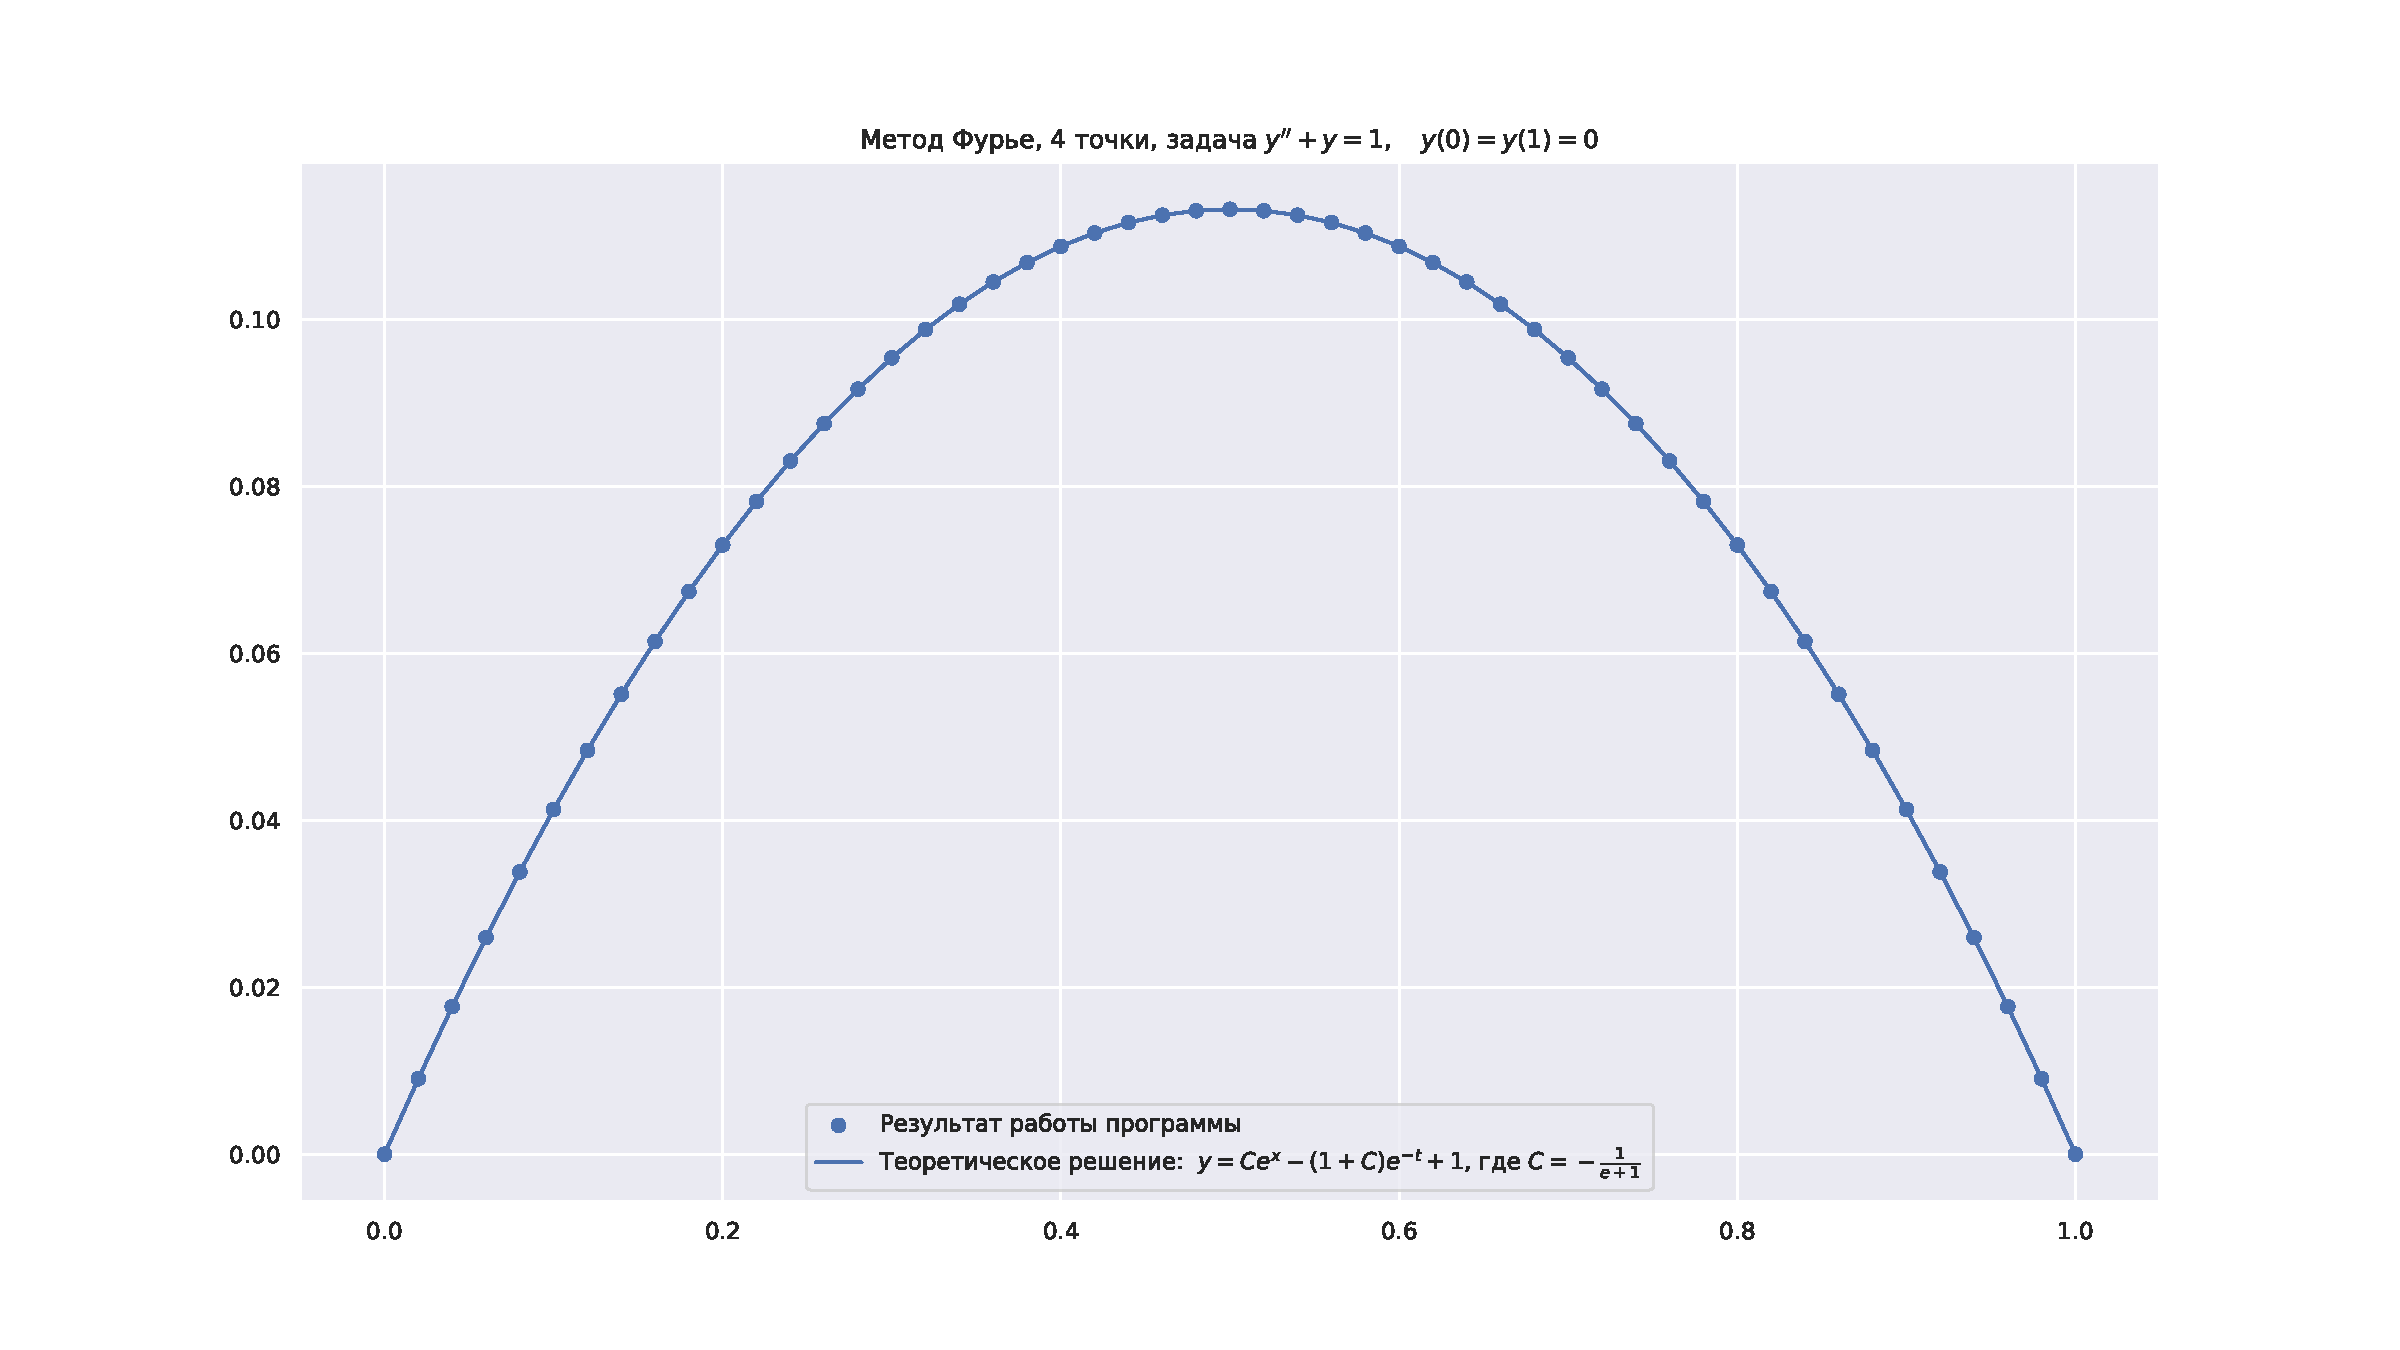
\includegraphics[scale=0.4]{figs/f50p1f1.pdf}
    \caption{Результаты теста на корректность для $p=1$, метод Фурье}
\end{figure}

\begin{figure}
    \centering
    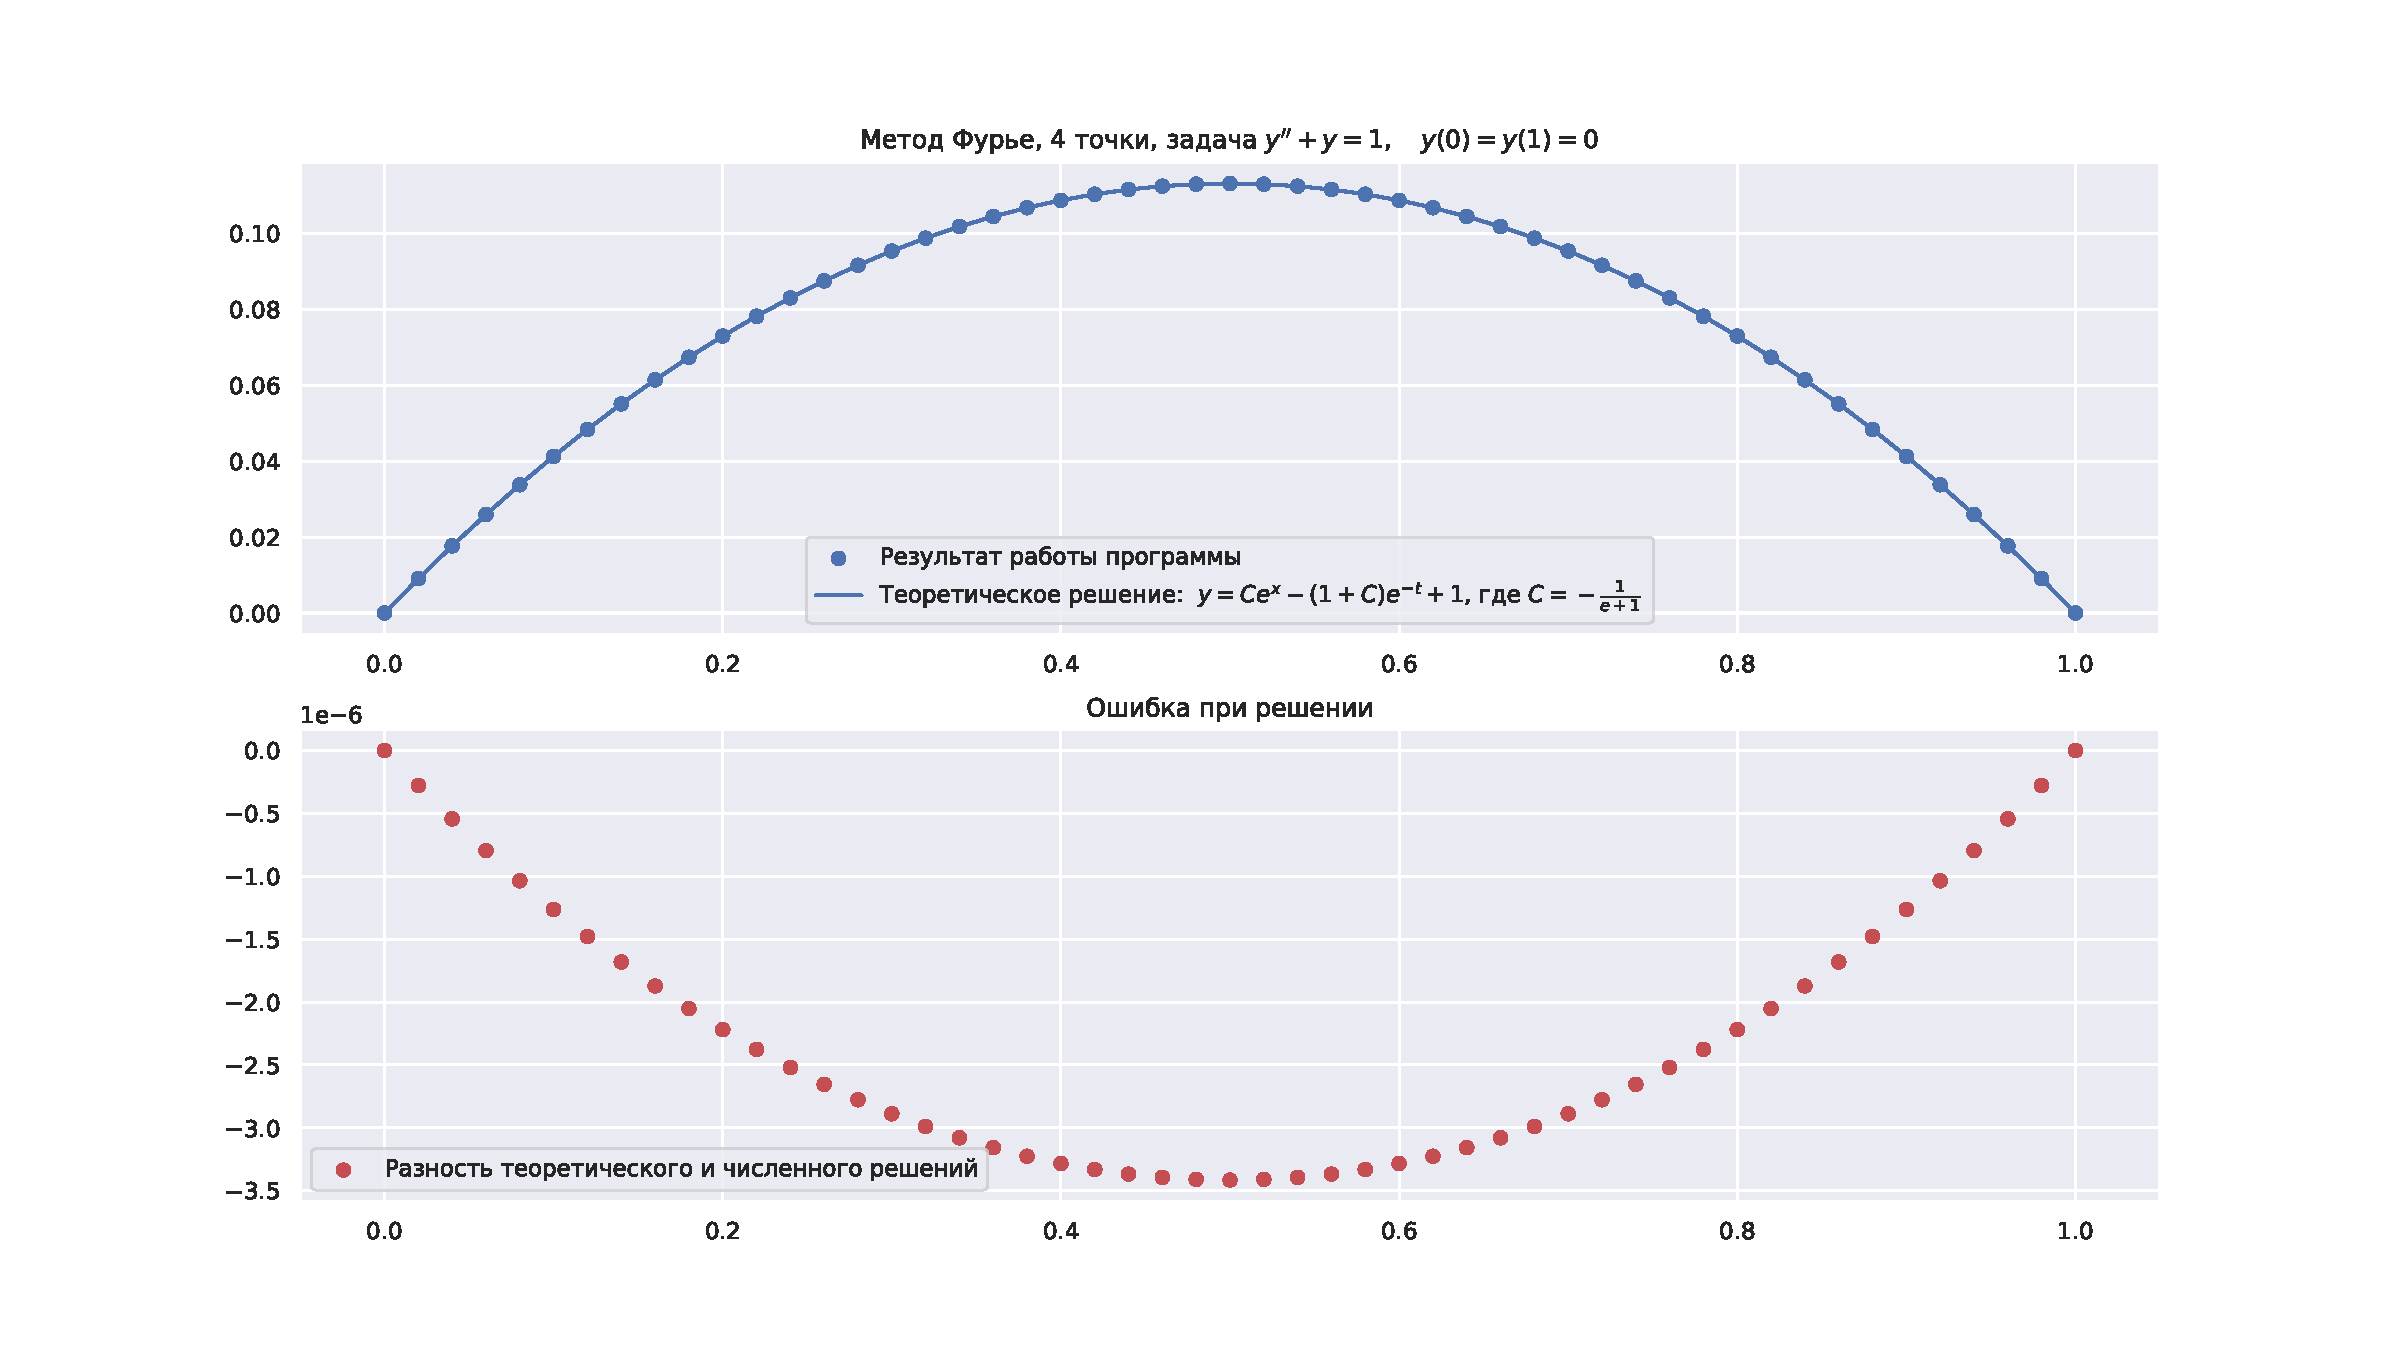
\includegraphics[scale=0.4]{figs/s50p1f1.pdf}
    \caption{Результаты теста на корректность для $p=1$, метод прогонки}
\end{figure}

\end{document}